% #########################################################################
% ##                          FITXER: 5_markov.tex                       ##
% ##        Contingut: Explicació i execució cadenes de Markov           ##
% #########################################################################

\documentclass[../main.tex]{subfiles}

% ------------------------------------------------------------
% Paquets específics
% ------------------------------------------------------------
\usepackage{paquets_format}
%\usepackage{almutils}

% ------------------------------------------------------------
% Inici del document
% ------------------------------------------------------------
\begin{document}

% ============================================================
% CAPÍTOL: Modelització ambs Cadenes de Markov
% ============================================================

\chapter{Modelització amb Cadenes de Markov} \label{ch:Cadenes de Markov}

\section{Aplicació de les cadenes de Markov en meteorologia}

Les cadenes de Markov són eines estadístiques basades en processos estocàstics que permeten modelitzar l'evolució dels estats d’un sistema en què el següent, depèn de l'actual. Aquest mètode ha demostrat ser útil per representar una gran varietat de sistemes reals amb estats discrets, com ara sistemes de cues, sistemes d’inventari o mercats de productes \parencite{liu2010application}, així com per modelitzar variables meteorològiques categòriques com l’ocurrència o absència de precipitació de precipitació, intervals de temperatura o l'estat del cel \parencite{gabriel1962markov}.  

El funcionament de les cadenes de Markov es basa en la idea que la transició entre estats segueix una probabilitat condicionada. És a dir, la probabilitat que el sistema estigui en un estat $j$ en el temps $t+1$ depèn només de l'estat $i$ en el temps $t$, i es pot escriure com:

\begin{equation}
\mathbb{P}(X_{t+1} = j \mid X_t = i)
\label{eq: notació probabilitat transició}
\end{equation}

Sent $X$ una variable aleatòria que representa l'estat del sistema.

Aquesta probabilitat es defineix segons l'equació \cref{eq: definició probabilitat condicionada}, on donats dos possibles esdeveniments $A , B$ , la probabilitat condicionada que es doni $A$, sabent que s'ha donat $B$ es defineix com: 

\begin{equation}
\mathbb{P}(A \mid B) = \frac{\mathbb{P}(A \cap B)}{\mathbb{P}(B)}
\label{eq: definició probabilitat condicionada}
\end{equation}


Quan es disposa d’una sèrie temporal discreta, et pot calcular, empíricament, la probabilitat de cada transició entre estats comptant el nombre de vegades que es produeix una seqüència concreta. Això permet estimar les probabilitats de transició com: 

\begin{equation}
    \mathbb{P}(X_{t+1} = j \mid X_t = i) = \frac{\text{nombre de transicions de } i \rightarrow j}{\text{nombre total de vegades que es troba l’estat } i}
    \label{calcul prob transició concreta}
\end{equation}



Aquest conjunt de probabilitats condicionades es representen en forma de matriu de transició on cada fila correspon a l'estat actual i cada columna al següent. Sent $i$ , $j$ , $k$  tres possibles estats del sistema, les diverses probabilitats condicionades es veurien com la següent matriu:

\begin{equation}
P =
\begin{bmatrix}
P_{ii} & P_{ij} & P_{ik} \\
P_{ji} & P_{jj} & P_{jk} \\
P_{ki} & P_{kj} & P_{kk}
\end{bmatrix}
\label{eq: def matriu transició}
\end{equation}


on $P_{xy} = \mathbb{P}(X_{t+1} = y \mid X_t = x)$, sent $x,y$ qualsevol dels estats possibles ($i,j,k$), representa la probabilitat condicionada que el sistema es trobi en l’estat $y$ en el temps $t+1$, donat que en el temps $t$ estava en l’estat $x$.

Tot i que existeixen cadenes de Markov d’ordre superior, en què l’estat futur depèn de més d’un estat anterior (per exemple, $\mathbb{P}(X_{t+1} \mid X_t, X_{t-1})$ en una cadena de segon ordre), aquestes impliquen una cost computacional superior i, per aquesta raó, sovint es prefereixen les cadenes de primer ordre, especialment quan l’objectiu és capturar la dependència immediata \parencite{inm2004}.

Aquest mètode, ha estat utilitzat en meteorologia per simular sèries binàries de precipitació (pluja / no pluja), com explica \textcite{inm2004}. Aquest enfocament permet predir seqüències com, la durada mitjana de períodes secs o humits, el primer dia de pluja després d'una ratxa seca, entre d'altres. A partir de les probabilitats de transició, es poden generar sèries temporals dels estats. 


\section{Plantejament del problema amb sèries de Markov}

Una primera aproximació a l'estudi de la predicció de series temporals amb cadenes de Markov s'ha de fer per força amb variables categòriques, ja que aquesta metodologia es basa en un càlcul de probabilitats discretes.  Per això,  es proposa fer el càlcul de la probabilitat del tipus de precipitació basant-se en la discretització de la temperatura en diferents rangs , tal com es fa a, \textcite{lefebvre2019markov}, en el qual aquesta estratègia s’utilitza per modelitzar i predir variacions mensuals de temperatura a Itàlia.

Prenent aquest enfocament com a referència, s’han definit tres intervals de temperatura, cadascun associat a un tipus de precipitació:

\begin{equation}
\text{Tipus de precipitació} =
\begin{cases}
\text{Neu (N)} & \text{si } T < 1^\circ\text{C} \\
\text{Aiguaneu (A)} & \text{si } 1^\circ\text{C} \leq T \leq 2^\circ\text{C} \\
\text{Pluja (P)} & \text{si } T > 2^\circ\text{C}
\end{cases}
\label{eq: Definició estats N,A,P}
\end{equation}


En aquest cas, les dades dades són horàries i provinents de l’estació meteorològica de la Bonaigua, tal com s’indica al \cref{ch:Obtencio i tractament de dades}. Tanmateix s'han considerat exclusivament els mesos corresponents a l’hivern climatològic (novembre, desembre, gener i febrer), amb l’objectiu de garantir la presència d’una distribució representativa entre les tres categories. Aquesta elecció evita augmentar el desbalanceig de la categoria de pluja en els mesos més càlids, que dificultaria l'aplicació de la metodologia.

Les probabilitats de transició s’han calculat a partir de les dades dels hiverns compresos entre les temporades 2000–2001 i 2022–2023. L’hivern 2023–2024 s’ha establert com a conjunt de test per tal de validar la capacitat predictiva del model. Les figures \Cref{fig:markov1} i \Cref{fig:markov2} mostren, respectivament, l’evolució de la temperatura i la classificació en categories durant aquest període.

\begin{figure}[H]
    \centering
    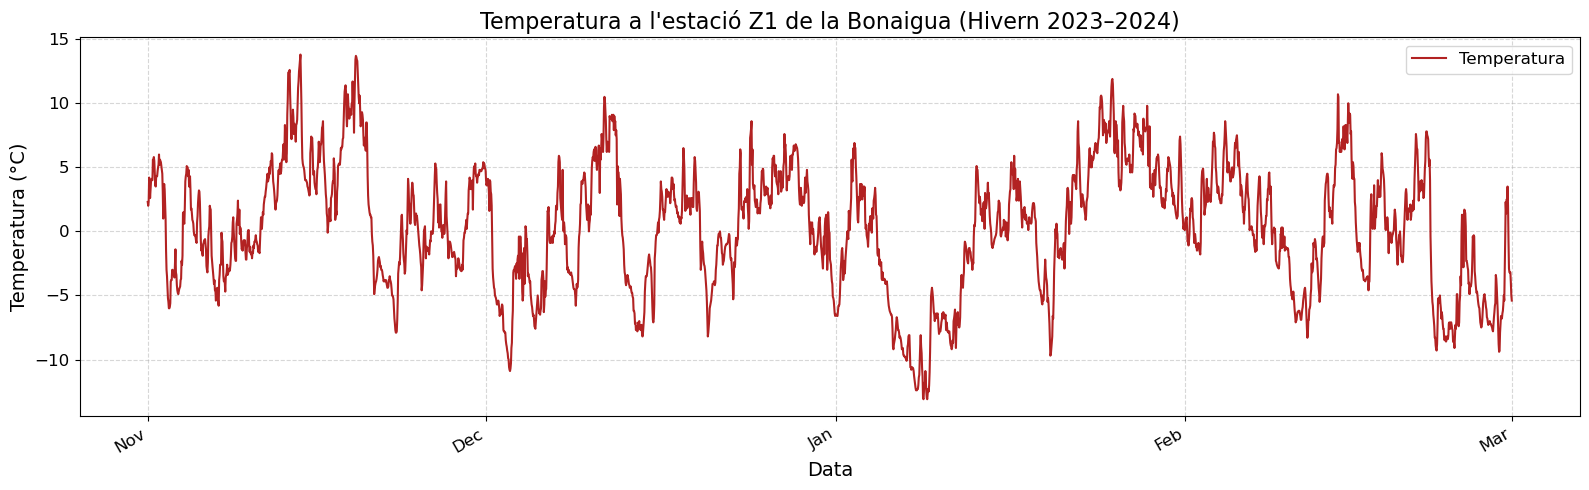
\includegraphics[width=\textwidth]{figures/markov/1.png}
    \caption{Evolució de la temperatura a l'estació de la Bonaigua durant l’hivern 2023–2024.}
    \label{fig:markov1}
\end{figure}

\begin{figure}[H]
    \centering
    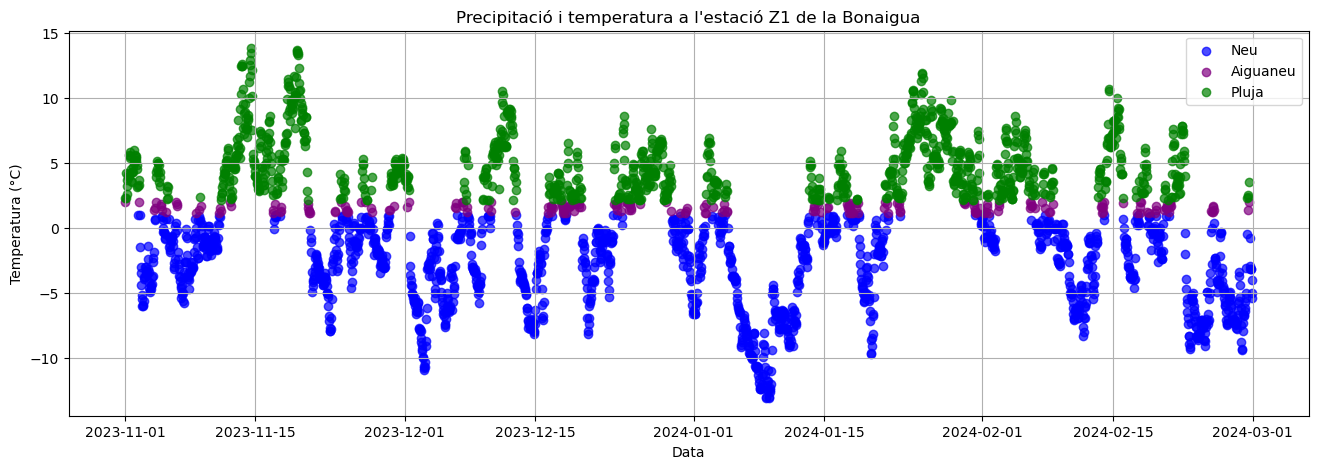
\includegraphics[width=\textwidth]{figures/markov/2.png}
    \caption{Discretització de la temperatura en categories de precipitació a l'estació de la Bonaigua durant l’hivern 2023–2024.}
    \label{fig:markov2}
\end{figure}

\section{Predicció i resultats del model de Markov}

Amb les dades històriques, s’han calculat les probabilitats de transició entre estats i sintetitzat en una matriu (\Cref{tab:matriu transicio}), que són la base del model.

\begin{table}[H]
    \centering
    \renewcommand{\arraystretch}{1.3}
    \begin{tabular}{cccc}\toprule
        
        \textbf{Estat anterior $\rightarrow$ Actual} & \textbf{Neu (N)} & \textbf{Aiguaneu (A)} & \textbf{Pluja (P)} \\\midrule
        
        \textbf{Neu (N)}      & 0.9717 & 0.0218 & 0.0065 \\
        \textbf{Aiguaneu (A)} & 0.2809 & 0.4872 & 0.2320 \\
        \textbf{Pluja (P)}    & 0.0175 & 0.0745 & 0.9080 \\ \bottomrule
        
    \end{tabular}
    \caption{Matriu de transició estimada a partir del conjunt d'entrenament. Les files representen l’estat de precipitació a l’hora anterior, i les columnes l’estat a l’hora actual.}
    \label{tab:matriu transicio}
\end{table}

Abans de fer la simulació, les probabilitats de la matriu ja permeten anticipar alguns comportaments. L’estat de neu (N) i el de pluja (P) tenen una alta persistència, amb valors superiors al 90\%, cosa que indica que, un cop s’hi entra, és molt probable que es mantinguin. En canvi, l’aiguaneu (A) és menys estable, i actua com a estat de transició: té gairebé la meitat de probabilitat de quedar-se, un 40\%, i una probabilitat de mes del 20\%  de passar tant a neu com a pluja. Les transicions directes entre neu i pluja són molt baixes, fet que té sentit si es té en compte que representen situacions extremes separades per un marge tèrmic, i que la temperatura es una variable contínua. Aquests salts implicarien un canvi brusc de temperatura en menys d'una hora, cosa que és molt poc probable.

Seguidament, s’ha dut a terme una simulació estocàstica de l’evolució dels estats a partir de la matriu de transició. A cada pas de temps, donat l’estat actual en l’instant \( t \), es genera l’estat següent \( t+1 \) mitjançant un procés de mostreig aleatori, seguint la distribució de probabilitats associada a aquell estat en la matriu de transició. 

Cal destacar que en cada pas s’utilitza sempre l’estat real observat en \( t \) per determinar la distribució de probabilitats del següent pas, i no l’estat simulat anterior, ja que l’objectiu és generar una seqüència de prediccions a partir de la sèrie real. La \cref{fig:markov3} mostra la seqüència de prediccions generada, que s’ha comparat amb la sèrie real per valorar la capacitat del model de capturar els patrons temporals.


\begin{figure}[H]
    \centering
    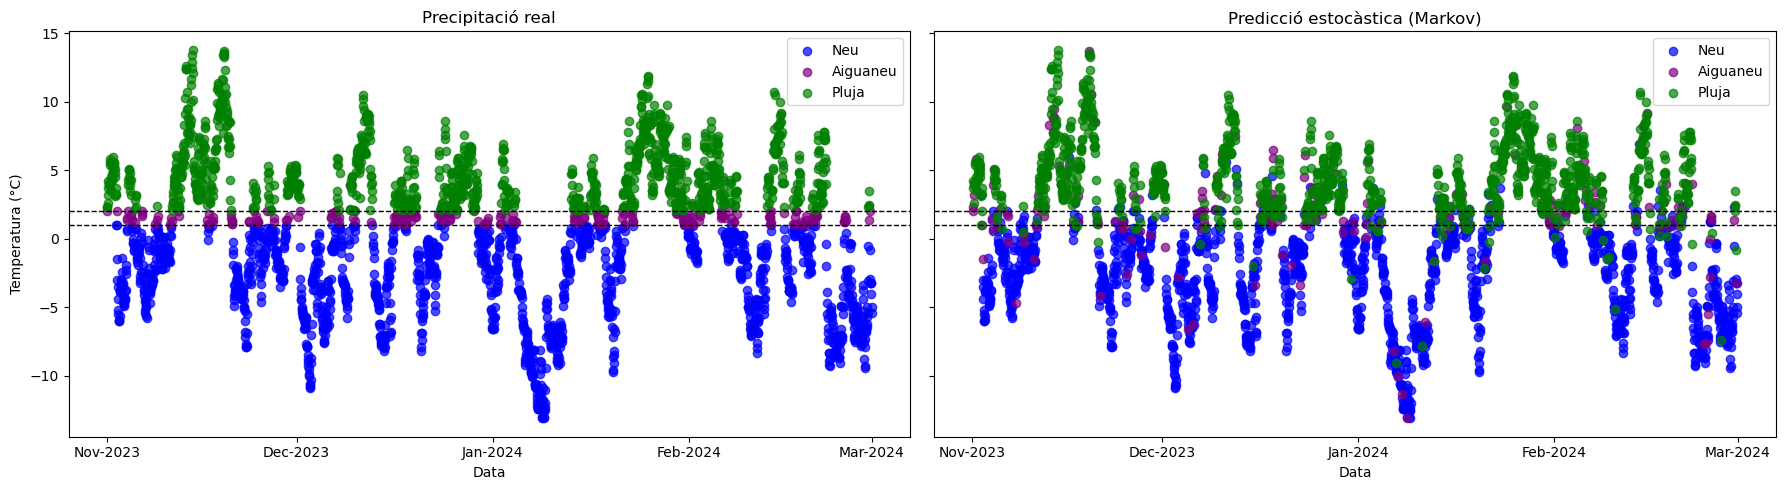
\includegraphics[width=\textwidth]{figures/markov/3.png}
    \caption{Comparació entre la sèrie real (esquerra) i la predicció generada pel model de Markov (dreta).}
    \label{fig:markov3}
\end{figure}

La matriu de confusió de la \Cref{fig:markov4} resumeix els encerts i errors de classificació respecte als valors reals observats. El model presenta un alt nivell d’encert en l’estat de neu (1.443 encerts) i pluja (979 encerts), mentre que l’estat intermedi d’aiguaneu presenta una menor taxa de classificació correcta (60 encerts sobre 219 casos).

\begin{figure}[H]
    \centering
    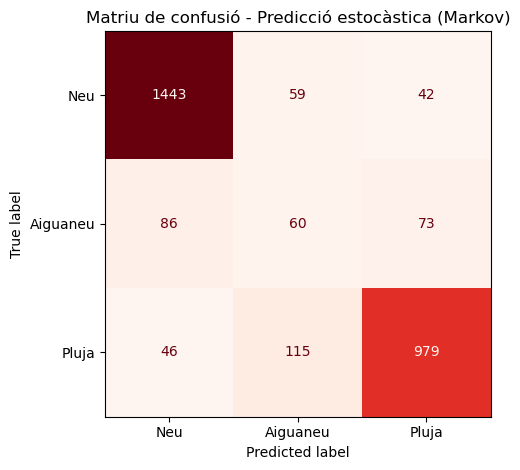
\includegraphics[width=0.45\textwidth]{figures/markov/4.png}
    \caption{Matriu de confusió del model de Markov.}
    \label{fig:markov4}
\end{figure}

Les \Cref{fig:markov5} i \Cref{fig:markov6} permeten analitzar la distribució de freqüències i el valor de \textit{recall} per classe. Pel que fa a les freqüències, s'observa que el model tendeix a mantenir la proporció entre real i predit, però respecte al  \textit{recall} per classes, els resultats mostren valors elevats per a neu (prop del 93\%) i pluja (al voltant del 86\%), mentre que per a aiguaneu el valor cau per sota del 30\%.


\begin{figure}[H]
    \centering
    \begin{minipage}[b]{0.48\textwidth}
        \centering
        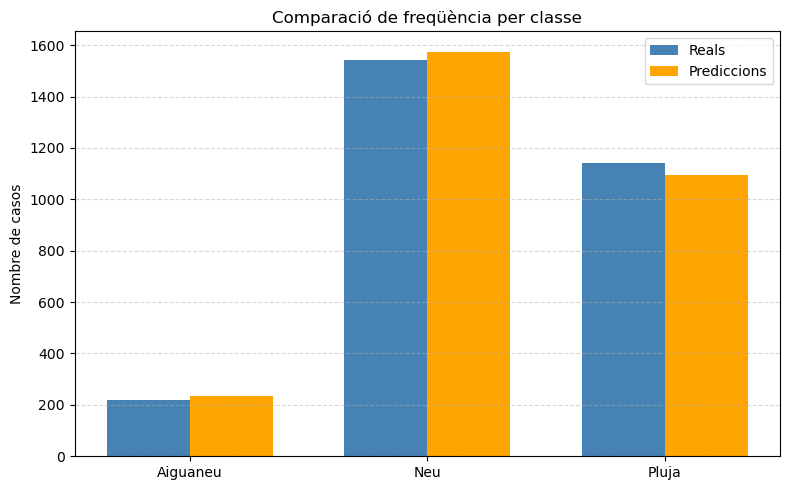
\includegraphics[width=\textwidth]{figures/markov/5.png}
        \caption{Comparació de freqüències entre classes reals i predites.}
        \label{fig:markov5}
    \end{minipage}
    \hfill
    \begin{minipage}[b]{0.48\textwidth}
        \centering
        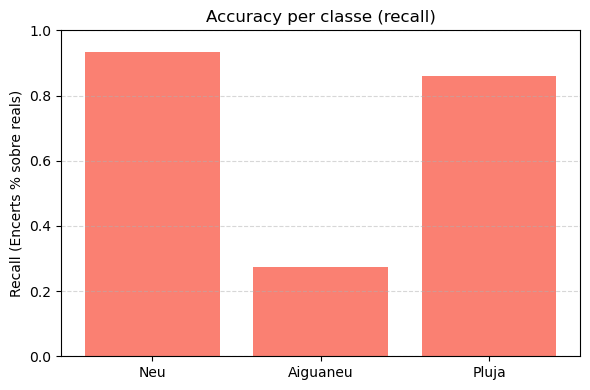
\includegraphics[width=\textwidth]{figures/markov/6.png}
        \caption{Valor de \textit{recall} per classe.}
        \label{fig:markov6}
    \end{minipage}
\end{figure}


En conjunt, els resultats mostren que el model de Markov és capaç de capturar amb eficàcia els patrons generals i els estats dominants del sistema (Neu i Pluja). Malgrat això, les transicions entre estats similars, com ara entre neu i aiguaneu o entre aiguaneu i pluja, es prediuen amb dificultat i menys certesa. Aquestes limitacions poden atribuir-se a la proximitat dels llindars de classificació, que és bàsicament  1 grau, i al fet que el model no té memòria mes enllà d'un estat ni incorpora altres variables meteorològiques que podrien ajudar.

% ------------------------------------------------------------
% Fi del document
% ------------------------------------------------------------
\end{document}
